\documentclass[conference]{IEEEtran}
\IEEEoverridecommandlockouts
% The preceding line is only needed to identify funding in the first footnote. If that is unneeded, please comment it out.
\usepackage{cite}
\usepackage{amsmath,amssymb,amsfonts}
\usepackage{algorithmic}
\usepackage{graphicx}
\usepackage{textcomp}
\usepackage{xcolor}
\def\BibTeX{{\rm B\kern-.05em{\sc i\kern-.025em b}\kern-.08em
    T\kern-.1667em\lower.7ex\hbox{E}\kern-.125emX}}
\begin{document}

\title{COMP9517 Individual Project}

\author{\IEEEauthorblockN{ Lijun Zhong}
\IEEEauthorblockA{\textit{University of New South Wales} }
}

\maketitle

\begin{abstract}
This project selects an appropriate classification method based on a given image data set to perform classification work, and compares the impact of different method applications.
\end{abstract}

\begin{IEEEkeywords}
plant image, image processing, classification 
\end{IEEEkeywords}

\section{Introduction and Background}
Plants can be said to be the most closely related group of organisms on earth, and correct identification of plant types is the prerequisite for most basic production and life content. The purpose of this personal project is to correctly classify plants such as Arabidopsis and tobacco based on image analysis. After extracting features based on the given 227 images, select appropriate classification methods for experiments and summarize them.
\section{Method (implementation)}

\subsection{Project Structure}
This experiment is generally divided into three parts: the first is the image preprocessing part, the second is the data set segmentation part, the third step is the image feature extraction part, the fourth step is the model building prediction part, and the fifth and final step is Evaluate the model part. In the whole project, the idea of controlling variables is mainly used to analyze and compare different methods of the same step. Please refer to Figure 1 for the specific framework.
\begin{figure}[htbp]
\centerline{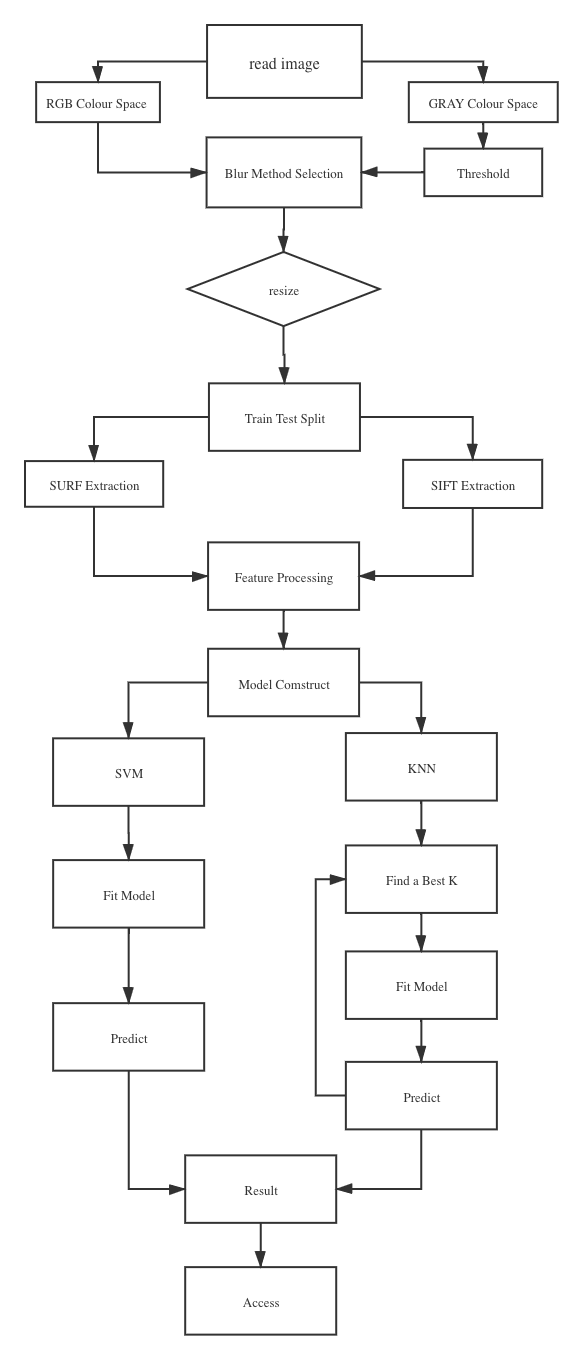
\includegraphics[scale=0.4]{P1.png}}
\caption{Project flow chart}
\label{fig1}
\end{figure}

\subsection{Preprocessing}
\subsubsection{Resizing and formating}
In order to get a faster result, the size of the picture is smaller. The purpose of this is to increase the running speed and be more accurate in the recognition results under ideal conditions Grasp. Due to the large size of the RGB image, but on the other hand, we also know that a picture can also be reflected by its grayscale image. Therefore, the grayscale conversion of the target image can reduce the design complexity and operating efficiency. Although the gray scale conversion can effectively reduce the size of the picture, the 256 gray scale picture still brings some time consumption to the processing, so it is necessary to reduce the gray scale greatly while keeping the original image information unchanged. Generally, the characteristic parameters of each direction are calculated and averaged, so that a comprehensive Indicators to identify the image.


\subsubsection{Preprocessing-Blur}
 Through the observation of the images in the data set, it is found that the overall resolution of the images in the Arabidopsis data set is reduced, compared with the tobacco picture, which is much clearer, which leads to too much detail and too much noise in the picture, which will affect the extraction and analysis of data features. Therefore, we use a variety of fuzzy algorithms to achieve blur. By reducing the performance of details, the number of occurrences of noise is actually reduced.
\paragraph{GaussianBlur Filter}
Gaussian blur is the resulting Gaussian function of the blurred image. It is an effect of widely used graphics software, which usually reduces image noise and reduces details. The visual effect of this blur technology is similar to a smooth blur, viewing the picture through a semi-transparent screen, which is significantly different from the effect of bokeh in the usual lighting of the focusing lens or the shadow of the object. 
\paragraph{MedianBlur Filter}
The median filter method is a non-linear smoothing technique, which sets the pixel value of each pixel to the median of all pixel values in a certain neighborhood window of that point. Statistical sorting filter, the median value has a good suppression effect on salt and pepper noise (with maximum and small value characteristics), and the effect is that the flaws in the image are smoother.
\paragraph{MeanBlur Filter}
Mean filtering is a typical linear filtering algorithm. The size of the template can cover the neighboring pixels around the target pixel (this project With the target pixel as the center of the surrounding 8 pixels, that is, remove the target pixel itself) and the center pixel, and then multiply the value in the template with the pixel value of the original image under it, and take the average of the sum of these products Instead of the original target pixel value.


\subsection{Feature extraction-Kmeans}
This project uses the idea of K-Means algorithm to distinguish the features in the picture. For a given feature sample set, the feature sample set is divided into K clusters according to the distance between the feature samples. For the K-Means algorithm, the first thing to pay attention to is the choice of k value. 
\subsection{Feature extraction-SURF}
\begin{itemize}
\item Scale space extreme value detection: construct Gaussian pyramids, Gaussian difference pyramids, and detect extreme points.
\item Key point positioning: remove the influence of small contrast and edges on extreme points.
\item Determine the direction of key points: Use gradient histogram to determine the direction of key points.
\item Key point description: block the image area around the key point, calculate the gradient histogram within the block, generate feature vectors, and describe the key point information.
\end{itemize}



\subsection{Classifications}
This project has conducted experiments on the following classifiers and selected an optimal choice. For specific parameters, please refer to Section III:
\subsubsection{Support vector machines (SVM)}
Support Vector Machine (SVM) is a powerful classification and regression technique that can maximize the prediction accuracy of the model without overfitting the training data. SVM is particularly suitable for analyzing data with a large number of predictive variable fields. The working principle of SVM is to map data to a high-dimensional feature space, so that even if the data is not linearly separable, the data points can be classified. After that, the characteristics of the new data can be used to predict the group to which the new record belongs.

\subsubsection{K-Nearest Neighbours (KNN)}
When there is a training sample set, and each data in the sample set has a label. After inputting new data without labels, compare each feature of the new data with the corresponding features of the data in the sample set, and then extract the classification label of the data with the most similar features (nearest neighbor) in the sample set. Generally, we only select the top K most similar data in the sample set. Finally, the classification of the k most similar data that appears the most times is selected as the classification of the new data.


\section{Experiment}
\subsection{Experimental setup}
\subsubsection{Metrics with threshold or RGB image}
Table 1 is the metrics comparation applying threshold grayscale, set no bluring method, set KNN's k equal to 3 .
In this case, I choose RGB as the default color space.
\begin{table}[htbp]
\caption{Metrics with different color space}
\begin{center}
\begin{tabular}{|c|c|c|c|c|}


\hline
Color Space& SVM-Acc &SVM-Rec&KNN-Acc &KNN-Rec\\
\hline
GRAY& 0.927536&0.884737 &0.9420290  &0.9436842\\
\hline
RGB& 0.942029 &0.927368 &0.9530435  &0.9473684\\
\hline


\end{tabular}
\label{tab1}
\end{center}
\end{table}



\subsubsection{Metrics with differen blur method}
Table 2 is the metrics comparation applying different filter as image preprocessing, applying GRB color space, set set KNN's k at 3 .
In this case, we could see that, there is a great increase when applying Gaussian filter or Median filter. And we may have a inspect on the filtered image as comparation.


\begin{table}[htbp]
\caption{Metrics with different Filter}
\begin{center}
\begin{tabular}{|c|c|c|c|c|}


\hline
Fileter& SVM-Acc &SVM-Rec&KNN-Acc &KNN-Rec\\
\hline
Not apply& 0.942029 &0.882353 &0.8985507  &0.8733032\\
\hline
Gaussian& 0.956522&0.953684 &0.9855072  &0.9900000\\
\hline
Mean& 0.956522 &0.953684 &0.9565217  &0.9700000\\
\hline
Median& 0.973684  &0.954382 &0.9912281  &0.9800000\\
\hline


\end{tabular}
\label{tab2}
\end{center}
\end{table}

In this case, there are demands to check the images marked with keypoints (As shown in Figure 2 ):
It can be observed that after filtering is used, the feature points of the read picture are more concentrated on the leaves of the plant itself. The performance of the Gaussian filter is much more obvious than that of the median filter. The leaves on both sides of the plant in the picture are in the original It is difficult to read the key points in the picture, and the picture after Gaussian processing has achieved good results.
\begin{figure}[htbp]
\centerline{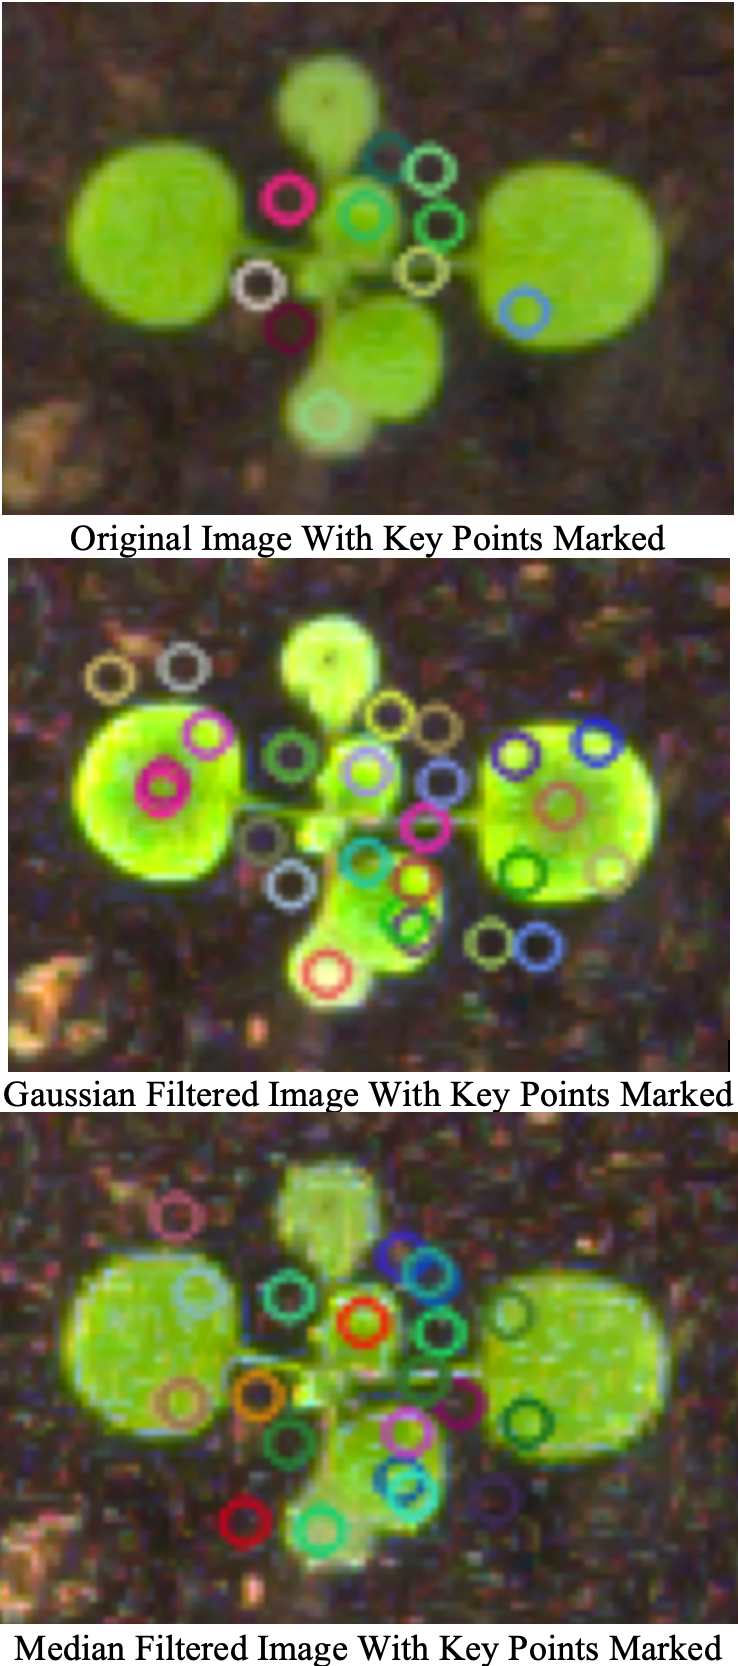
\includegraphics[scale=0.4]{P2.png}}
\caption{Filtered images marked with keypoints}
\label{fig2}
\end{figure}

\subsubsection{KNN's K value selection}
In practical applications, the K value generally takes a relatively small value. For example, the cross-validation method (in simple terms, part of the sample is used as the training set and the other part is used as the test set) to select the optimal K value.


\begin{figure}[htbp]
\centerline{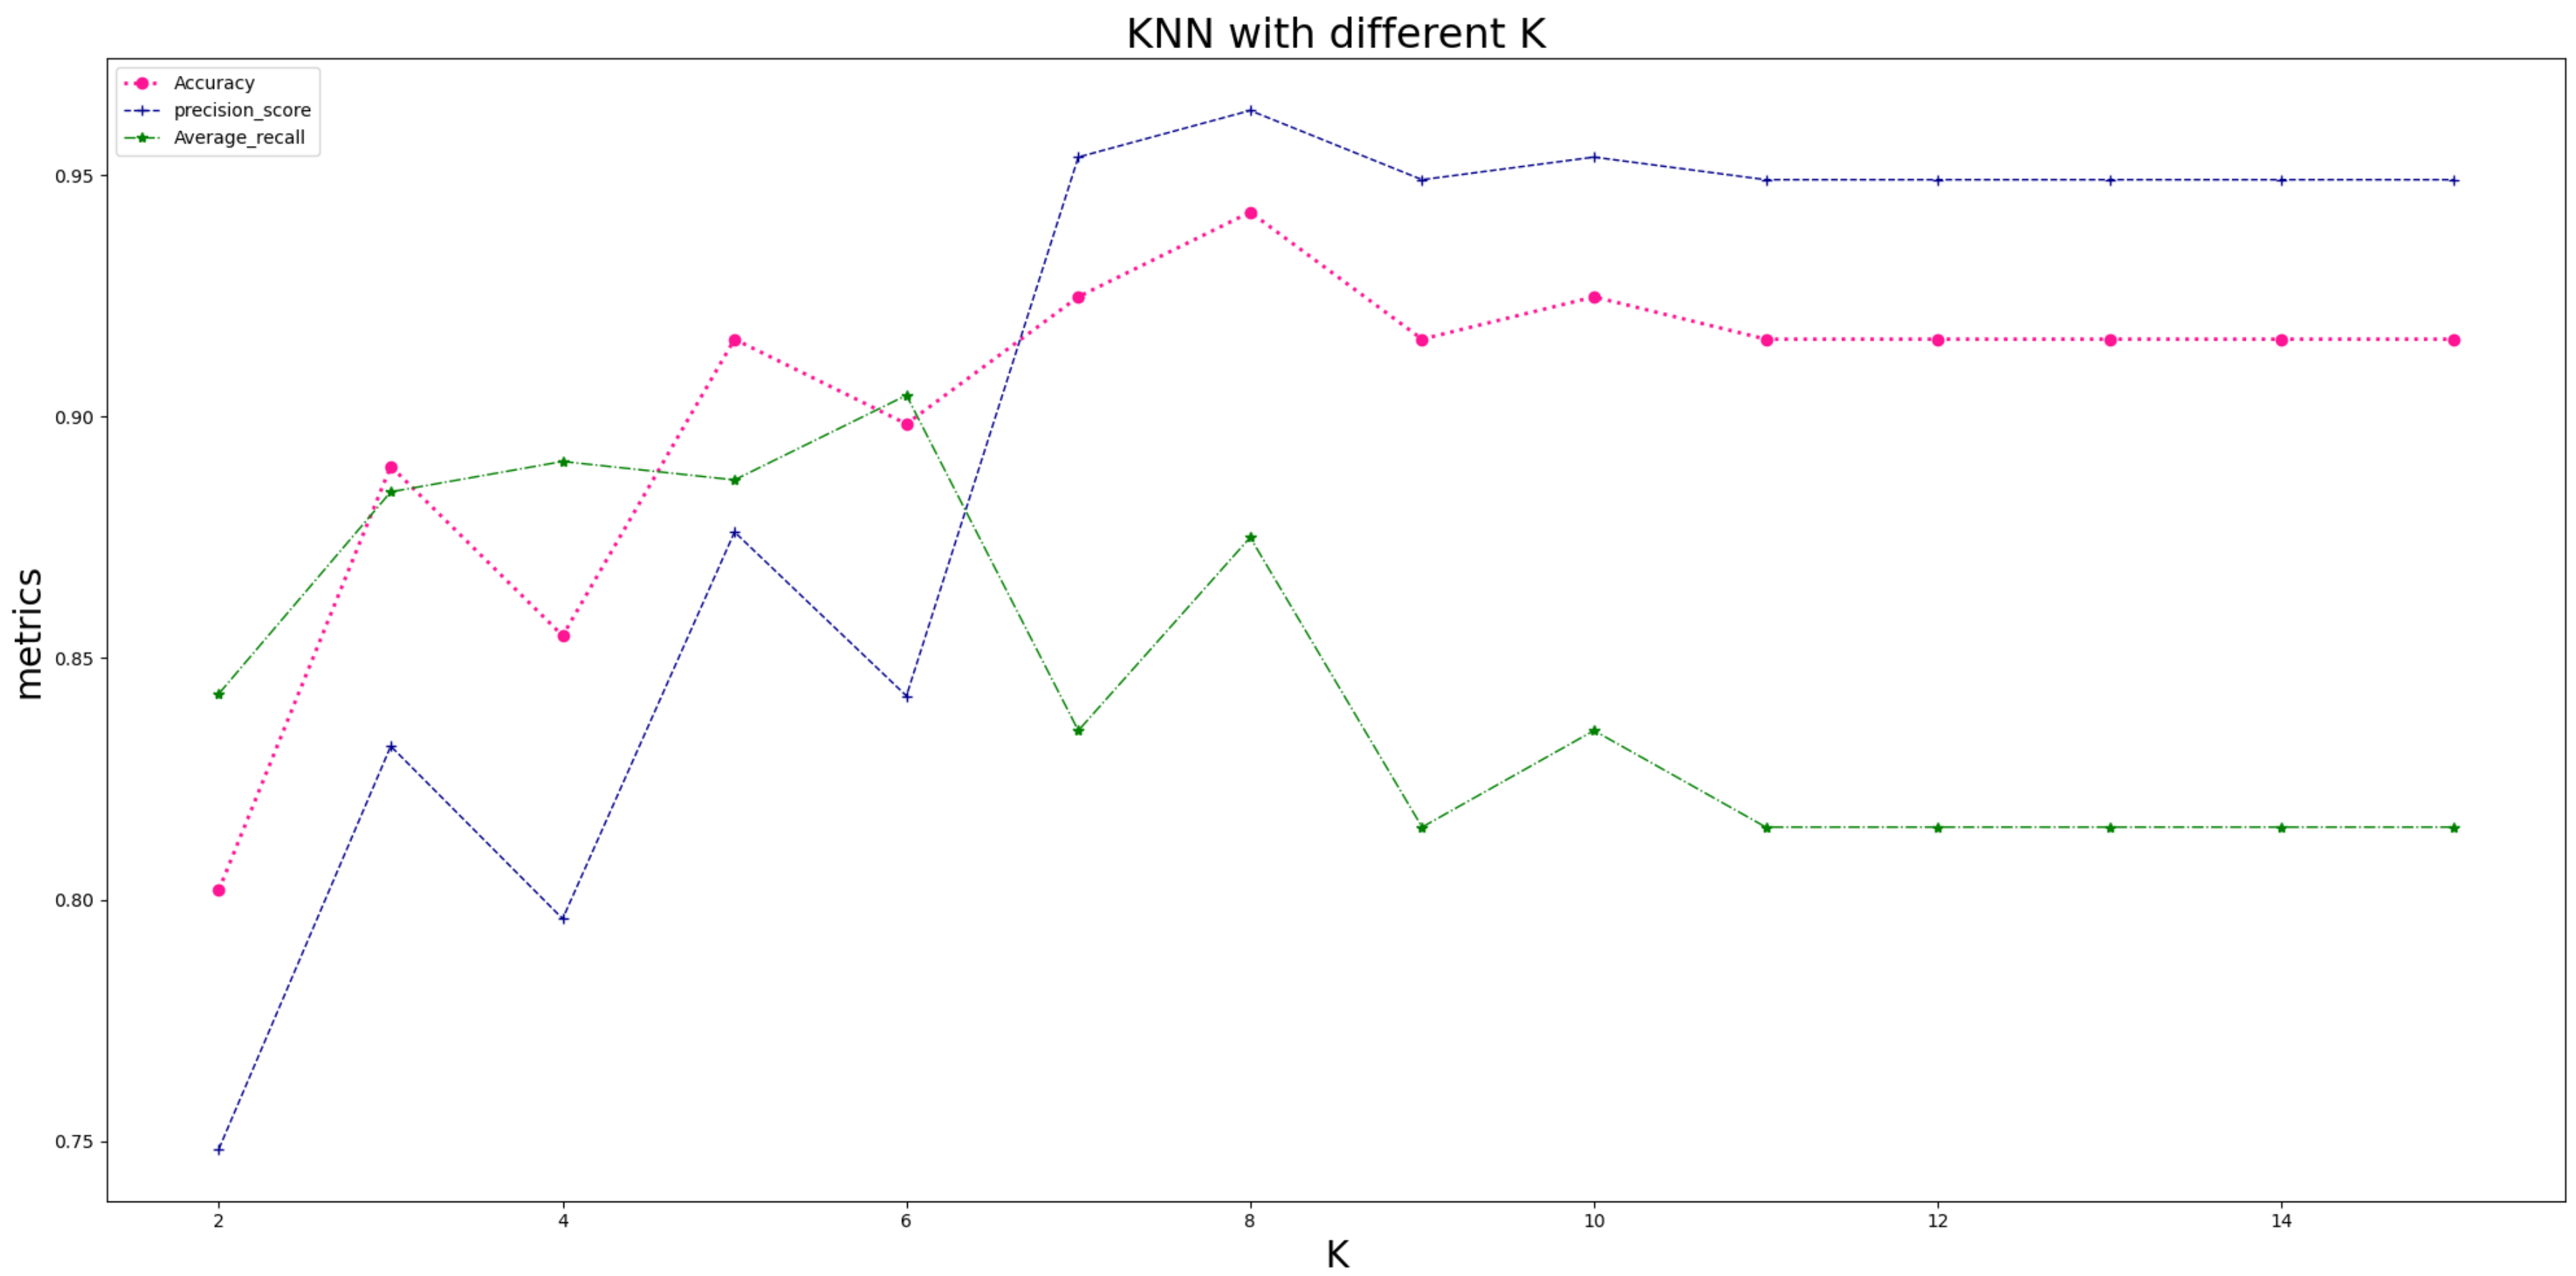
\includegraphics[scale=0.15]{P3.png}}
\caption{Metrics of different K in KNN model.}
\label{fig3}
\end{figure}

It can be seen from Figure 3 that when the K value is 8, the accuracy and recall rate are highest, and the slope increases to both sides showing a downward trend, and the K value is selected as 8.




\section{Results and Discussion}
\subsubsection{Metrics selection}
The important parameters of the evaluation model are metrics. Table III shows the three indicators of the two models SVM and KNN (the optimal K has been taken). In this comparison, in order to reduce the probability of a single experiment and the lack of data The “pseudo-overfitting phenomenon” caused by contingency to the accuracy of the model adopts a kind of cross-validation method, and randomly divides the data set many times to find the average of the three metrics: 

\begin{table}[htbp]
\caption{Metrics of models with 10-Cross Validation}
\begin{center}
\begin{tabular}{|c|c|c|c|c|}



\hline
CLF &Accuracy&Precision &Recall&Average Time\\
\hline
SVM&0.956522 &0.949882   &0.931561 & 27.2\\
\hline
KNN&0.9710145 &0.9609729   &0.9609729& 48.7 \\
\hline


\end{tabular}
\label{tab3}
\end{center}
\end{table}

\subsubsection{Evaluation}
it can be seen that the KNN has set the optimal K. Its performance is slightly better than SVM, but the overall running time is longer. It can be said that these two models have their own advantages, but considering the reference of large-scale data sets, the accuracy of the KNN model is not more obvious. On the contrary, due to the increase in time and space complexity of calculation, it may cause the problem of calculation overload. Therefore, it is a more reasonable choice to choose SVM.\
\subsubsection{Reflection}
\begin{itemize}
\item In subsequent experiments, it should be considered whether the part of the picture with too high signal-to-noise ratio can be cropped to improve the effective information rate of the matrix and reduce the computational cost.
\item Introduce more classifiers and parameters for horizontal comparison to show the comparative advantages of classifiers.
\item Select different classifiers according to different feature extraction methods, such as HOG+SVM is more suitable for face recognition, and explore a faster and more accurate combination
\end{itemize}



\begin{thebibliography}{00}
\bibitem{b1} Jean-Michel Pape and Christian Klukas. Utilizing machine learning approaches to improve the prediction of leaf counts and individual leaf segmentation of rosette plant images. In S. A. Tsaftaris, H. Scharr, and T. Pridmore, editors, Proceedings of the Computer Vision Problems in Plant Phenotyping (CVPPP), pages 3.1-3.12. BMVA Press, September 2015.
\bibitem{b2} Singh A, Ganapathysubramanian B, Sarkar S, Singh A. Deep learning for
plant stress phenotyping: trends and future perspectives. Trends Plant
Sci. 2018;23:883–98.


\end{thebibliography}



\end{document}
